\section{Introduction}
The goal of this chapter is to introduce {\bibtex}, the course of
events leading to {\bibtex} \chapref{sec:why_bibtex_came_to_be}, what
{\bibtex} is \chapref{sec:principles_of_bibtex}, how {\bibtex} is used
in principle \chapref{sec:practice_of_bibtex} and how {\bibtex} is
used in practice \chapref{sec:how_bibtex_is_used_today}.


\section{Why {\bibtex} came to be}
\label{sec:why_bibtex_came_to_be}

The advent of {\TeX} has been a game changer for scientific writing,
witness the number of articles written in {\TeX} (or derivatives such
as {\LaTeX}).  For instance, on arXiv.org, nearly all articles are
formatted with \LaTeX.  Apart from being grateful to Donald Knuth
for providing a robust system for scientific articles, writers can
also be thankful that {\TeX} has given the basis for Oren Patashnik
and Leslie Lamport to create {\bibtex} for managing scientific
bibliographies.

Before the wake of {\bibtex}, references were managed entirely by hand
and required a lot of labor.  For instance, nearly half of Mary-Claire
van Leunen's book, \textit{A Handbook for
  Scholars}~\cite{leunen1992_handbook}, is dedicated to citing,
managing and writing references, \ie, 150 pages out of 335 pages
(excluding the index).  Likewise, a significant fraction of Umberto
Eco's book, \textit{How to Write a Thesis}~\cite{eco1985_thesis}, is
also dedicated to managing and citing references and to ensuring a
proper bibliography.  All this manual labor has almost been made
obsolete by {\bibtex}.

Even more, {\bibtex} entries are now readily available online, and so
the practical problem of bibliographic references is now solved, in
principle.

\section{What is {\bibtex}}
\label{sec:principles_of_bibtex}

In the same spirit as {\LaTeX}, {\bibtex} is a simple software tool
for managing references in scientific writing, using an ASCII file to
write the references.  Inside this file, the components of each
reference are specified, such as the author, title, year and what kind
of medium (such as a book or article) was used.

Depending on the forum, there are differences in how references should
be cited and be written.  Each publisher has a mandatory setup.  The
specific set of rules a publisher has is referred to as a
\newdef{bibliography style} or \newdef{citing style}.

When using {\bibtex} on a document, {\bibtex} cites according to the
selected bibliography style, ensures the formatting in the reference
list, and ensures that only relevant entries are included.  The
references are labeled consistently in the document according to the
citing style, the labels are used when a reference is cited and these
labels allows the reader to quickly find the reference in the
bibliography, as illustrated in \figref{fig:bibtex_example_alpha}.

Today, {\bibtex} has also enabled huge online resources with
references, automated extraction tools, sharing of references and easy
version control.  The {\bibtex} format is originally designed for use
with {\LaTeX}, but it has plugins for other formats as
well~\cite{bibtex_resource}.

\begin{figure}
  \centering
  
\includegraphics[width=0.8\textwidth]{bibtex-styles-ex-acm}
  \caption{{\bibtex} output using ACM citing style which uses numbers to
    index entries}
\label{fig:bibtex_example_acm}
\end{figure}

\section{How {\bibtex} is used in principle}
\label{sec:practice_of_bibtex}

\subsection{Macro-use}

A {\bibtex} file consists of entries each corresponding to a
reference, such an article or a book.  Each entry in turn contains
meta information about the reference, through tags that specify the
kind of meta information such as the author or title.  Also, quite
commonly, a file will contain a lot of shortenings for text fragments
that are reused.

To select the desired style the command
${\backslash}bibliographystyle$ is used, for example
${\backslash}bibliographystyle\{alpha\}$.  The style in turn controls
the formatting and how the references are labeled, as can be seen on
\figref{fig:bibtex_example_acm} and \figref{fig:bibtex_example_alpha}
where the labels are different, the abbreviation of author names are
different and some of the visual formatting is different.

To build a {\LaTeX}-document with {\bibtex} references in it, one
first runs the $latex$ command (or one of the derivatives) to produce
(among other things) an aux file.  The aux file contains auxiliary
information from the {\LaTeX}-compiler.  Then run the $bibtex$ command
which uses the aux file to find the entries in use and to give them
labels according to the reference style in use.  The output from
{\bibtex} is a bbl file with the formatted references, which is then
used by subsequent runs by {\LaTeX}, so the document will have labels
a the appropriate places and an bibliography in accordance with the
labels.


\subsection{Micro-use}

Inside a {\bibtex} file the format itself is fairly simple. At the
main level we got $@STRING$, $@PREAMBLE$, $@COMMENT$ and $entries$.
$@STRING$ is for shortenings that can be used later in the {\bibtex},
$@PREAMPLE$ is for defining how to format the text and $@COMMENT$ is
for comments and $entries$.  The $entries$ correspond to the different
medium types, such as $@ARTICLE$, $@BOOK$ and $@PROCEEDINGS$, which in
turn contains the relevant tags for the given entry.  For each entry
type, there are a specification of tags relevant to the given medium
where some of them are mandatory. For instance for an $@ARTICLE$ the
tags $author$, $title$, $year$ and $journal$ are mandatory and
supplementary information such as the $pages$ for the article and
$volume$ of the journal can be added.  For ease of use {\bibtex}
provides predefined strings for the months: $jan$, $feb$, $mar$ and so
on.

Tags and entries are case insensitive. The literal content
(\newdef{text}) needs to be enclosed in either \{ and \} or quotes and
numbers can be written without.  $@STRING$ shortenings has to be
without quotes and curly brackets.  Concatenation of $@STRING$ and/or
text is done using \#~\cite{bibtex_resource}.  {\bibtex} is designed
to ignore unknown entries and tags, so it allows additional
information.  An example {\bibtex} file can be seen in
\figref{fig:bibtex_example}

\begin{figure}
  \centering
  \begin{small}
\begin{verbatim}
@String{JFP = "Journal of Functional Programming"}
@String{OUP = "Oxford University Press"}

@Article{abadi1991_substitutions
  author =      "Mart\'{\i}n Abadi and Luca Cardelli
                 and Pierre-Louis Curien
                 and Jean-Jacques L\'evy",
  title =       "Explicit substitutions",
  journal =     JFP,
  year =        1991,
  volume =      1,
  number =      4,
  pages =	"375--416",
  note =	"A preliminary version was presented at the Seventeenth
                 Annual {ACM} Symposium on Principles
                 of Programming Languages
                 (POPL 1990)"
}

@InBook{leunen1992_handbook,
  author =       "Mary-{C}laire van Leunen",
  title =        "A Handbook for Scholars",
  publisher =    OUP,
  year =         1992,
  pages =        "9--45,154--268"
}
\end{verbatim}
  \end{small}
  \caption{{\bibtex} example}
\label{fig:bibtex_example}
\end{figure}

When citing inside {\LaTeX} the desired key from the {\bibtex} is used
inside the ${\backslash}cite$, for example if one has a reference
named $some\_article$ then the reference is used by writing:
${\backslash}cite\{some\_article\}$.  To link the document and the
bibliography together the command ${\backslash}bibliography$ is used
together with a parameter for the {\bibtex} file, for example:
${\backslash}bibliography\{mybib\}$.

\begin{figure}
  \centering
  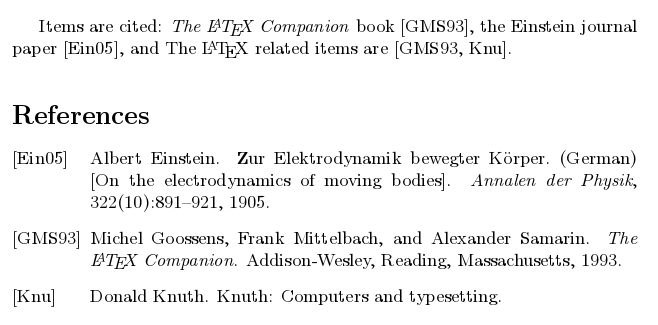
\includegraphics[width=0.8\textwidth]{bibtex-styles-ex-alpha}
  \caption{{\bibtex} output using alpha citation style which uses
    author names and year to index entries}
\label{fig:bibtex_example_alpha}
\end{figure}


\section{How {\bibtex} is used in practice}
\label{sec:how_bibtex_is_used_today}

{\bibtex} is to this day routinely used by researchers, witness that
almost all online resources for finding references provide {\bibtex}
output.  Many online databases are widely used to look up entries,
which has also given rise to a lot of ways to identify articles, such
as: arXiv numbers, DOI and ISSN.

Since {\bibtex} is capable of only printing the references used in a
{\LaTeX}-document most people start using {\bibtex} as a database
having a complete file with the references they have used.  A lot of
people also find it practical to use their {\bibtex} file as a way to
keep track of what they read.

That {\bibtex} ignores unknown tags is also widely used, both for de
facto standards and to add additional information that the format does
not specify, such as arXiv numbers, DOI and ISSN.  It is so widely
used that is is common to see article search engines make have tags
that are not specified by {\bibtex} and there is libraries that
provide citing styles that make use of these tags.


\section{Summary and conclusions}
\label{sec:about_conclusion}

{\bibtex} is a product of the advent of {\TeX} and the
need for managing references, {\TeX} made it possible to automate,
through this simple format.  {\bibtex} provides a simple way to manage
references and it is fairly flexible and thus allows for useful de
facto standards.  The inside of a {\bibtex} file is simple and
intuitive, dividing the entries in to types corresponding to the
medium it represents and having tags relevant to that medium.
{\bibtex} has become widely used and given rise to useful de facto
standards and tools to assist with bibliographic references.

{\bibtex} have been a game changer, and is something for every
scientific author to be happy about, so has {\bibtex} solved the
problem of bibliographic references? It would seem so, had it not been
for Murphy's Law, as detailed in the next chapter.


%\remark{(Note to self:) should probably have half an eye on things
%  like: `G{\"o}del', when working with it}
%
%\remark{(Note to self:) people may use booktitle where title is
%  appropriate edition: The edition of a book---for example,
%  ``Second''. This should be an ordinal, and should have the first
%  letter capitalized, as shown here; the standard styles convert to
%  lower case when necessary~\cite{bibtex_description}.}
%
%\remark{http://tug2000.tug.org/TUGboat/Articles/tb24-1/patashnik.pdf}f